\documentclass[11pt]{article}
\usepackage{amsmath, amssymb}
\usepackage{geometry}
\usepackage{hyperref}
\usepackage{graphicx}
\usepackage{booktabs}
\geometry{margin=2.5cm}
\graphicspath{{../plots/}}
\emergencystretch=2em

\newcommand{\ket}[1]{|#1\rangle}
\newcommand{\Pop}{\hat{P}}
\newcommand{\Oedge}{X_0 Z_1\cdots Z_{L-2} X_{L-1}}
\newcommand{\expv}[1]{\langle #1\rangle}
\newcommand{\cx}{\texttt{cx}}

\title{Why Topology Still Matters When the Measurement Is Not Noise Immune\\
\large Noise, chain length, and the optimal VQE depth}
\author{Seminar notes}
\date{\today}

\begin{document}
\maketitle

\begin{abstract}
The Kitaev-chain simulation is not noise immune in the NISQ sense: the state is
prepared by ordinary noisy gates, and the edge-string diagnostic is a long,
non-local measurement whose contrast is easily reduced by gate, readout, and
decoherence errors. Topology still matters because it changes the \emph{ideal}
many-body physics: the logical information is stored non-locally in two separated
Majorana edge modes, and the finite-size splitting between the two parity sectors
falls exponentially with chain length. The practical rule is therefore not
``make the circuit deeper.'' It is: use the \emph{shallowest adequately expressive}
ansatz depth. For the current $L=4$ study this was $r=2$; for larger $L$ the
minimum useful value of $r$ may increase, but every extra repetition also adds
$L-1$ more noisy CNOTs.
\end{abstract}

\section{What topology protects}

For even $L$, the Jordan--Wigner parity operator used in the code is
\begin{equation}
  \Pop=\prod_{j=0}^{L-1}Z_j .
\end{equation}
The Kitaev-chain Hamiltonian is
\begin{equation}
  H =
  -\frac{\mu}{2}\sum_j Z_j
  +\frac{t-\Delta}{2}\sum_j X_jX_{j+1}
  +\frac{t+\Delta}{2}\sum_j Y_jY_{j+1}.
\end{equation}
Every term contains either zero or two $X/Y$ operators, so $[H,\Pop]=0$. Parity
conservation itself is therefore a $\mathbb{Z}_2$ symmetry of the Hamiltonian,
not a separate miracle of topology.

Topology enters in a different way. In the topological phase, $|\mu|<2t$, the
chain supports Majorana modes at opposite ends. The two end modes form one
non-local fermion. A local perturbation acting near one end cannot fully measure
or split that non-local degree of freedom unless it effectively connects the two
ends or creates a parity-changing event. In a finite chain the two edge modes
overlap weakly, so the even/odd splitting is not exactly zero, but it is
exponentially small:
\begin{equation}
  E_0(L)
  \approx
  2t(1-\lambda^2)\lambda^L,
  \qquad
  \lambda=\frac{|\mu|}{2t}.
\end{equation}
This is the useful protection: topology suppresses the \emph{intrinsic}
Hamiltonian splitting as $L$ grows, while the bulk remains gapped away from the
critical points.

\section{Why this is not noise immune}

The phrase ``topologically protected'' is easy to overstate. It does not mean
that any laboratory implementation or any measurement circuit is immune to all
noise. In this project there are four separate reasons the measured signal is
not noise immune.

\paragraph{1. The chain is finite.}
At finite $L$ the Majorana wavefunctions overlap. The ideal splitting is small
in the topological phase, but it is not exactly zero. Increasing $L$ reduces this
overlap, but it does not remove device noise from the circuit used to prepare and
measure the state.

\paragraph{2. The VQE circuit is an ordinary noisy circuit.}
The topological Hamiltonian is simulated with standard qubits and standard gates.
The ansatz used in the code is
\begin{verbatim}
EfficientSU2(L, su2_gates=['ry'], entanglement='linear', reps=r)
\end{verbatim}
Each repetition adds a linear CNOT layer. Thus
\begin{equation}
  N_{\theta}=L(r+1),
  \qquad
  N_{\mathrm{CNOT}}=r(L-1).
\end{equation}
If each CNOT carries an error channel, the topological nature of the target state
does not stop those channels from acting. The noisy simulation in
\texttt{block4.py} correctly applies the channel after every transpiled \cx{}
gate.

\paragraph{3. Some noise violates the protecting symmetry.}
Phase damping is diagonal in the computational basis, so it commutes with
$\Pop$ and preserves parity. Amplitude damping and depolarizing noise do not:
they contain operations that change the local $Z_j$ eigenvalue and therefore can
flip the global parity. In the repository convention,
$c_j^\dagger c_j=(I+Z_j)/2$, so computational $\ket{0}$ is the occupied
single-site state; the important point is not whether a channel is described as
adding or removing a fermion, but that it changes fermion-number parity.

\paragraph{4. The measured topological diagnostic is non-local.}
The edge string
\begin{equation}
  O_{\mathrm{edge}}=\Oedge
\end{equation}
is the correct finite-size Majorana edge diagnostic, but it is a long Pauli
string. Long strings are fragile under measurement noise. Symmetric readout error
with bit-flip probability $\epsilon$ attenuates a weight-$L$ string roughly as
\begin{equation}
  (1-2\epsilon)^L .
\end{equation}
Dephasing can leave $\expv{\Pop}$ unchanged while still destroying the endpoint
coherence that the edge string needs. This is why Block 4 can show both facts at
once: parity may remain fixed under parity-preserving noise, while the
topological string signal decays.

\section{Why topology still matters}

The model is still important because it provides a passive physical layer of
protection that ordinary local qubits do not have. A local qubit stores
information in one local degree of freedom, so a local disturbance can directly
read or damage it. A Majorana pair stores information non-locally, so local
perturbations have exponentially small access to the encoded splitting when the
bulk gap is open and the chain is long.

That is not a replacement for error correction, calibration, or careful
measurement. It is a different starting point: the ideal Hamiltonian already
suppresses one important class of errors. The NISQ problem is that our present
simulation does not use native protected Majorana hardware. It synthesizes the
state with ordinary CNOTs, then measures a long string. The physics has
topological structure; the circuit implementation still has ordinary gate noise.

This is also why the model is useful as a benchmark. It lets us separate three
questions that are often mixed together:
\begin{enumerate}
  \item Does the ideal Hamiltonian have topological edge modes?
  \item Can a variational circuit prepare the corresponding ground state?
  \item Does a noisy device preserve enough contrast to measure the non-local
  diagnostic?
\end{enumerate}
The answer can be yes, yes, and only partially. That is a meaningful result, not
a contradiction.

\section{How increasing chain length changes the optimal reps}

Let
\begin{equation}
  S_{\mathrm{meas}}(L,r)
  =
  |\expv{O_{\mathrm{edge}}}|_{\mathrm{meas}}
\end{equation}
be the measured edge-string magnitude after preparing the state with
\texttt{reps}$=r$. A useful approximation is
\begin{equation}
  S_{\mathrm{meas}}(L,r)
  \approx
  S_{\mathrm{ideal}}(L,r)
  \exp[-\eta_{\mathrm{cx}}\,r(L-1)]
  \exp[-\eta_{\mathrm{ro}}\,L],
  \label{eq:signal_model}
\end{equation}
where $S_{\mathrm{ideal}}(L,r)$ is the noiseless expressibility of the ansatz,
$\eta_{\mathrm{cx}}=-\log(1-p_{\mathrm{cx}})\approx p_{\mathrm{cx}}$ is the
per-CNOT noise cost, and $\eta_{\mathrm{ro}}\approx -\log(1-2\epsilon)$ is the
readout cost per measured qubit. The constants depend on the channel, but the
structure is robust: expressibility improves with $r$, while noise worsens with
the total number of CNOTs, $r(L-1)$.

Equation~\eqref{eq:signal_model} gives the practical rule. Increasing the reps
from $r$ to $r+1$ is worthwhile only if
\begin{equation}
  \log\frac{S_{\mathrm{ideal}}(L,r+1)}
           {S_{\mathrm{ideal}}(L,r)}
  >
  \eta_{\mathrm{cx}}(L-1).
  \label{eq:marginal_rule}
\end{equation}
The left side is the expressibility gain from one more layer. The right side is
the extra noise cost of the additional $L-1$ CNOTs. As $L$ grows, the cost of one
extra repetition grows linearly. Therefore deeper circuits become harder to
justify at larger $L$.

\subsection*{What happened at $L=4$}

For the current $L=4$ depth scan, $r=1$ is under-expressive: the noiseless edge
string is essentially zero. At $r=2$, the ansatz first reaches the correct
topological state, and deeper circuits do not significantly improve the ideal
signal. Once the ideal signal has saturated, Eq.~\eqref{eq:marginal_rule} fails:
the numerator is near one, while the extra CNOT cost is positive. Thus the noisy
optimum is
\begin{equation}
  r_{\mathrm{opt}}=2
  \qquad
  (L=4,\ \mu=0,\ \text{current ansatz}).
\end{equation}
This is why the Week 9 result is described as the \emph{shallowest adequately
expressive depth}.

\begin{figure}[h]
  \centering
  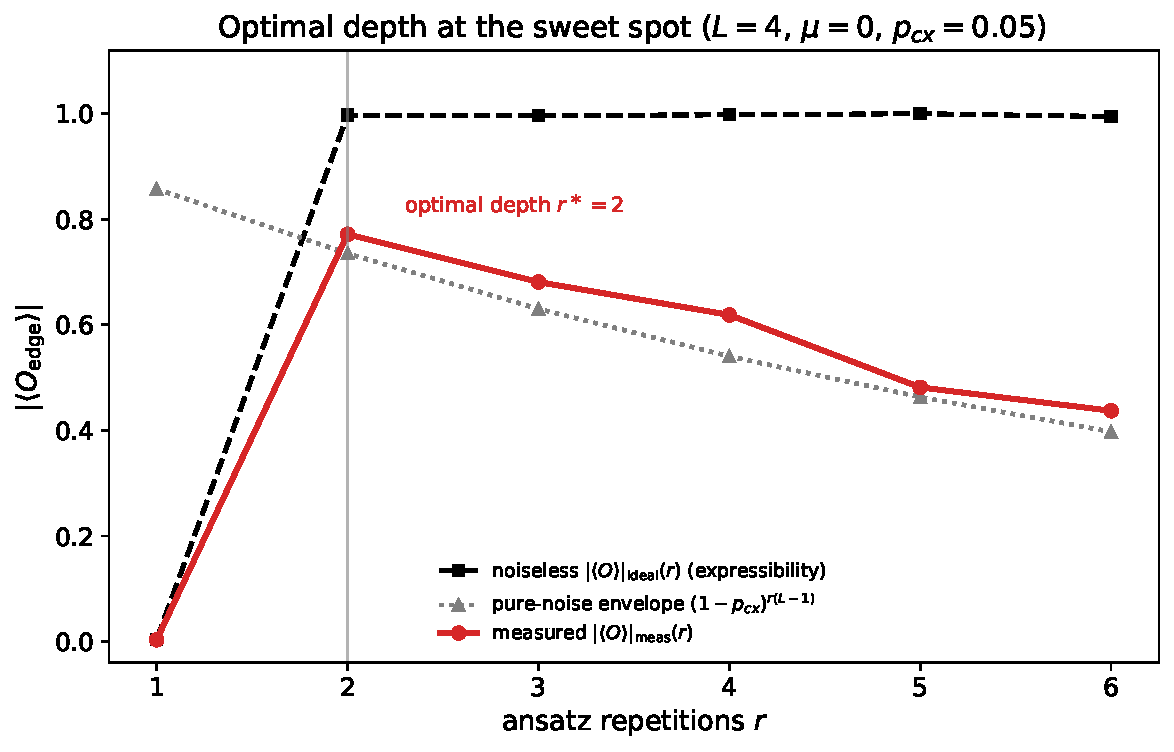
\includegraphics[width=0.78\linewidth]{block4_week9_depth_optimum.pdf}
  \caption{For $L=4$, the noiseless edge string has an expressibility threshold:
  $r=1$ fails, $r=2$ succeeds, and deeper circuits mainly accumulate CNOT noise.}
  \label{fig:depth_optimum}
\end{figure}

\subsection*{Should $r$ increase when $L$ increases?}

Usually, the minimum expressive depth should be expected to stay the same or
increase with $L$, not decrease. Larger chains contain more bonds, more
variational parameters, more parity constraints, and a longer non-local string.
Near the critical points $|\mu|=2t$, the correlation length grows, so the ground
state is harder to represent accurately. A larger $r$ may therefore be needed to
clear the same energy, fidelity, parity, and edge-string tolerances.

But there is no universal formula such as $r=L/2$ for this hardware-efficient
ansatz. The required depth depends on the ansatz, the phase point $\mu$, the
target tolerance, and the optimizer. Deep in the gapped topological phase, a
small number of repetitions may remain enough for the small system sizes we can
simulate. Close to criticality, or if high global fidelity is required across a
longer chain, the needed $r$ can grow.

The correct definition is empirical and validation-based:
\begin{equation}
  r_{\mathrm{expr}}(L,\mu)
  =
  \min\left\{
  r:
  \begin{array}{l}
  |E_{r}-E_{\mathrm{ED}}|\leq \delta_E,\\
  |\expv{\Pop}_{r}-1|\leq \delta_P,\\
  1-F_r\leq \delta_F,\\
  |S_{\mathrm{ideal}}(L,r)-S_{\mathrm{ED}}(L)|\leq \delta_S
  \end{array}
  \right\}.
\end{equation}
Then, when the ideal signal has threshold-like behavior, the noisy optimum is
approximately
\begin{equation}
  r_{\mathrm{opt}}(L,\mu)
  \approx
  r_{\mathrm{expr}}(L,\mu).
\end{equation}
In words: choose the first depth that passes the noiseless validation, and stop
there unless one more layer gives a visible ideal-signal gain larger than the
extra noise penalty in Eq.~\eqref{eq:marginal_rule}.

\section{The chain-length trade-off}

Increasing $L$ helps and hurts at the same time.

\begin{center}
\begin{tabular}{lll}
\toprule
Effect of increasing $L$ & Scaling tendency & Consequence\\
\midrule
Majorana overlap & $\sim (|\mu|/2t)^L$ & better intrinsic topological protection\\
Readout/string weight & $\sim (1-2\epsilon)^L$ & weaker measured string contrast\\
CNOT count at fixed $r$ & $r(L-1)$ & more accumulated gate noise\\
CNOT count if $r_{\mathrm{expr}}\sim L$ & $\sim L^2$ & severe noisy-depth penalty\\
\bottomrule
\end{tabular}
\end{center}

If $r_{\mathrm{expr}}(L)$ stays approximately constant, the circuit-noise envelope
still falls roughly as
\begin{equation}
  \exp[-\eta_{\mathrm{cx}}\,r_{\mathrm{expr}} L].
\end{equation}
If the expressive depth itself grows linearly with $L$, then
\begin{equation}
  N_{\mathrm{CNOT}}
  =
  r_{\mathrm{expr}}(L)(L-1)
  =
  O(L^2),
\end{equation}
and the measured signal can collapse much faster:
\begin{equation}
  S_{\mathrm{meas}}
  \sim
  \exp[-\mathrm{const}\cdot L^2].
\end{equation}
This is the central NISQ tension. Topology improves the ideal finite-size
physics with $L$, but the circuit used to demonstrate that physics becomes
longer and noisier with $L$.

\begin{figure}[h]
  \centering
  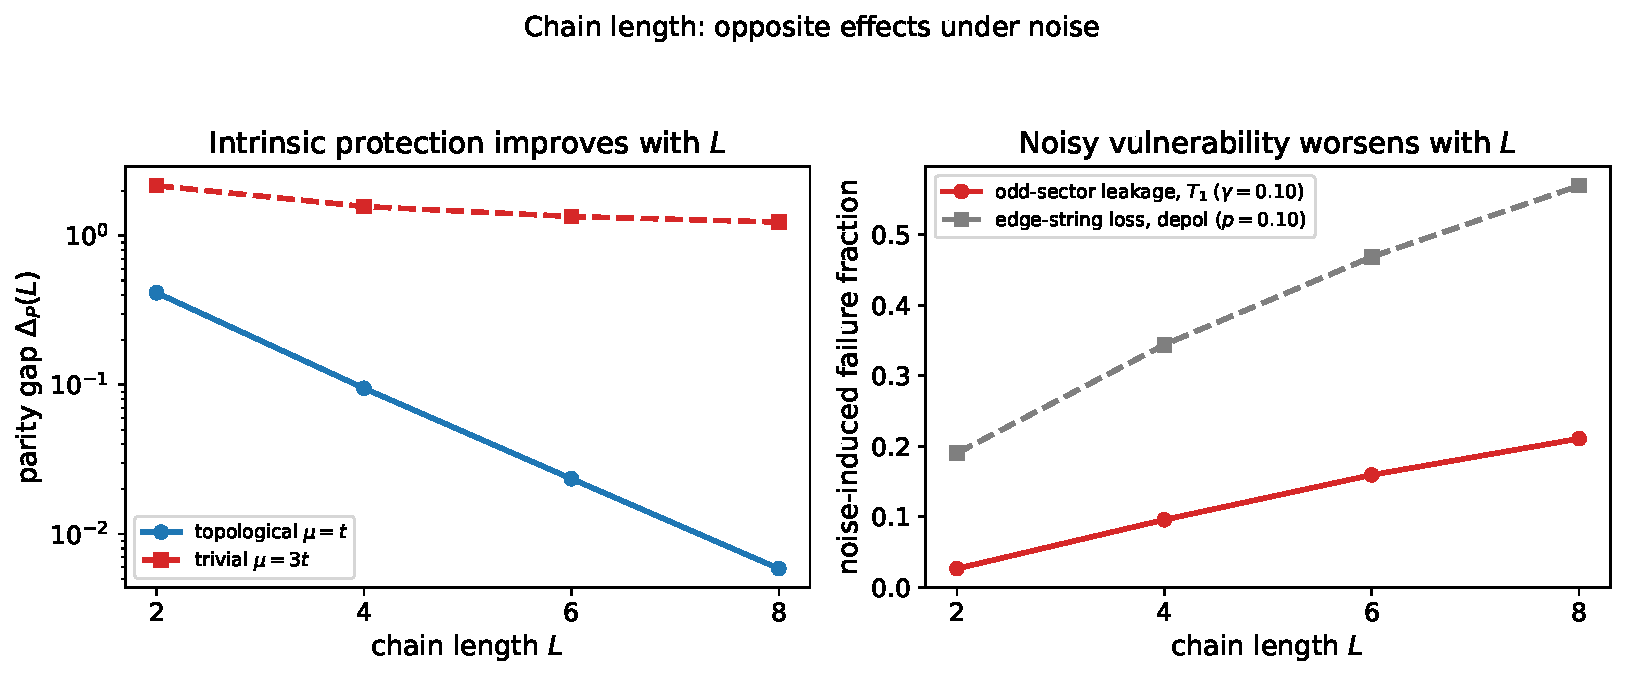
\includegraphics[width=0.95\linewidth]{block4_length_under_noise.pdf}
  \caption{Longer chains reduce the intrinsic topological splitting but increase
  exposure to noise in parity-changing and string-measurement channels.}
  \label{fig:length_tradeoff}
\end{figure}

\section{Practical answer for the project}

For $L=4$, the data justify $r=2$ as the optimum under CNOT noise because it is
the first depth that prepares the state. For larger $L$, do not assume $r=2$ will
always be enough, but also do not increase $r$ automatically. Run the same depth
scan at each target $L$. In the noisy study, choose
\begin{equation}
  r_{\mathrm{opt}}
  =
  \operatorname*{arg\,max}_{r\ \mathrm{passing\ validation}}
  S_{\mathrm{meas}}(L,r).
\end{equation}
With the threshold behavior observed here, this usually means the shallowest
depth that passes the ED/VQE validation and still gives the largest noisy
edge-string contrast.

If the depth scan says that $r_{\mathrm{expr}}$ grows quickly with $L$, then the
generic hardware-efficient ansatz is becoming the bottleneck. The right response
is not simply to keep adding layers. Better options are a more
Hamiltonian-inspired ansatz, parity-preserving gates, adiabatic/matchgate-style
state preparation, or restricting the NISQ demonstration to the largest $L$ for
which the edge-string contrast remains measurable.

\section{Summary}

\begin{itemize}
  \item The system is not noise immune because finite chains have overlap,
  simulated Majorana states are prepared by ordinary noisy gates, parity-violating
  channels can poison the protected sector, and the edge string is a long
  non-local measurement.
  \item Topology still matters because it stores information non-locally and
  suppresses the ideal even/odd splitting exponentially with $L$.
  \item The useful signal is approximately
  $S_{\mathrm{ideal}}(L,r)\exp[-\eta_{\mathrm{cx}}r(L-1)]$ times readout loss.
  \item Increasing $r$ is useful only while the ideal expressibility gain beats
  the extra CNOT-noise cost. At $L=4$, $r=2$ is enough; for larger $L$,
  $r_{\mathrm{expr}}$ may increase, but every added repetition costs $L-1$ more
  CNOTs.
  \item The correct rule is not ``larger $L$ means larger $r$''; it is ``larger
  $L$ requires a new depth scan, and the optimum is the shallowest validated
  depth.''
\end{itemize}

\begin{thebibliography}{9}
\bibitem{kitaev}
A. Kitaev,
\emph{Unpaired Majorana fermions in quantum wires},
\href{https://arxiv.org/abs/cond-mat/0010440}{arXiv:cond-mat/0010440}.

\bibitem{nayak}
C. Nayak, S. H. Simon, A. Stern, M. Freedman, and S. Das Sarma,
\emph{Non-Abelian Anyons and Topological Quantum Computation},
\href{https://arxiv.org/abs/0707.1889}{arXiv:0707.1889}.

\bibitem{alicea}
J. Alicea,
\emph{New directions in the pursuit of Majorana fermions in solid state systems},
\href{https://arxiv.org/abs/1202.1293}{arXiv:1202.1293}.
\end{thebibliography}

\end{document}
